%	file:		thesis.tex
%	author:	alex c. williams
%	updated:	6 May 2015

%	description:
%	this file provides a template for the mtsu computer science thesis.
%
%	NOTES
%	1. Chapter Headings should be bold in the "text" portion of the document.
%	- To fix:
%		1. add /textbf to each /chapter{} line
%		2. compile
%		3. remove \textnormal from the \thesection renew command.
%		4. compile
%
%	2. To change "Professor One" and etc., you need to modify the names in the complementary "committee_header.tex" file.

\documentclass[12pt, oneside]{book}

% Include these packages:
\usepackage[top=3.17cm, bottom=2.54cm, left=3.81cm, right=2.54cm]{geometry}	 % for margin requirements.
\usepackage{mathptmx}% http://ctan.org/pkg/mathptmx
\usepackage{setspace} % for double-spacing.
\usepackage{xifthen}%
\doublespacing
\usepackage{lipsum}
\usepackage{tocloft}
\usepackage{color}
\usepackage{array}
\usepackage{stfloats}
\usepackage[pdftex]{graphicx}
\usepackage{subcaption}
\usepackage[export]{adjustbox}
\usepackage{multirow}
\usepackage{url}
\usepackage{changepage}
\usepackage{floatrow}
\usepackage{titlesec}
\usepackage{fancyhdr}
\usepackage{chngcntr}
\usepackage{fancyhdr}

% -- Define code snippet configuration
\usepackage{listings}
\usepackage{color}

\definecolor{dkgreen}{rgb}{0,0.6,0}
\definecolor{gray}{rgb}{0.5,0.5,0.5}
\definecolor{mauve}{rgb}{0.58,0,0.82}

\lstset{frame=tb,
  language=Java,
  aboveskip=3mm,
  belowskip=3mm,
  showstringspaces=false,
  columns=flexible,
  basicstyle={\small\ttfamily},
  numbers=none,
  numberstyle=\tiny\color{gray},
  keywordstyle=\color{blue},
  commentstyle=\color{dkgreen},
  stringstyle=\color{mauve},
  breaklines=true,
  breakatwhitespace=true,
  tabsize=3
}

% -- Base Page Styling 
\floatsetup[table]{capposition=top}
\counterwithout{figure}{chapter}
\counterwithout{table}{chapter}
\setlength\textfloatsep{18mm}
\fancyhf{}
\fancyhead[R]{\thepage}

% -- Base Styling for Section/Subsection/Subsubsection --
\titlespacing{\section}{0pt}{\parskip}{-\parskip}
\titlespacing{\subsection}{0pt}{\parskip}{-\parskip}
\titlespacing{\subsubsection}{0pt}{\parskip}{-\parskip}

% Styling for Section Headers
\titleformat{\section}
{\normalfont\bfseries\filcenter}
{\textnormal\thesection}
{0cm}
{}

% Styling for Subsection Headers
\titleformat{\subsection}
{\normalfont\filcenter}
{\textnormal\thesubsection}
{0cm}
{}

% -- Stylize Subfigure Headings--
\newlength\Origarrayrulewidth
\renewcommand{\thesubfigure}{\Alph{subfigure}}
\newcommand{\Cline}[1]{%
 \noalign{\global\setlength\Origarrayrulewidth{\arrayrulewidth}}%
 \noalign{\global\setlength\arrayrulewidth{2pt}}\cline{#1}%
 \noalign{\global\setlength\arrayrulewidth{\Origarrayrulewidth}}%
}
\newcommand\Thickvrule[1]{%
  \multicolumn{1}{!{\vrule width 2pt}c!{\vrule width 2pt}}{#1}%
}

% -- Stylize the Table of Contents --
\renewcommand{\cfttoctitlefont}{\hfill\normalsize}
\renewcommand*\thesubsection{}
\renewcommand*\thesection{\textnormal}
\renewcommand*\thechapter{\Roman{chapter}.}
\renewcommand*\thepart{}
\renewcommand\cftchapfont{\mdseries}
\renewcommand{\cftchapleader}{\cftdotfill{\cftdotsep}}
\renewcommand\cftchappagefont{\normalfont}
\renewcommand\cftpartpagefont{\normalfont}
\renewcommand\contentsname{\hfill{\textbf{TABLE OF CONTENTS}}\hfill}
\renewcommand{\cftaftertoctitle}{\hfill}
\renewcommand{\cftbeforepartskip}{1.00em}

% -- Stylize Chapter Headings --
\makeatletter
\let\orig@chapter\@chapter
\def\@chapter[#1]#2{\ifnum \c@secnumdepth >\m@ne
                       \if@mainmatter
                         \refstepcounter{chapter}%
                         \typeout{\@chapapp\space\thechapter.}%
                         \addcontentsline{toc}{chapter}%
                                   {\textnormal{CHAPTER}~\protect\numberline{\thechapter}#1}%
                       \else
                         \addcontentsline{toc}{chapter}{#1}%
                       \fi
                    \else
                      \addcontentsline{toc}{chapter}{#1}%
                    \fi
                    \chaptermark{#1}%
                    \addtocontents{lof}{\protect\addvspace{10\p@}}%
                    \addtocontents{lot}{\protect\addvspace{10\p@}}%
                    \if@twocolumn
                      \@topnewpage[\@makechapterhead{#2}]%
                    \else
                      \@makechapterhead{#2}%
                      \@afterheading
                    \fi}
\makeatother

% Stylize List of Figures
\renewcommand*\listfigurename{LIST OF FIGURES}
\renewcommand{\cftloftitlefont}{\hfill\normalsize}
\renewcommand{\cftafterloftitle}{\hfill}
\setlength{\cftbeforeloftitleskip}{-3em}
\setlength{\cftafterloftitleskip}{-0.05em}
\renewcommand{\cftfigfont}{Figure }


\usepackage{titlesec}
\usepackage[tracking=true]{microtype}
\titleformat{\chapter}[display]
  {\vspace{-2.54cm}\normalsize}
  {\filcenter\textbf{\MakeUppercase{\chaptertitlename} \thechapter}}
  {\parskip}
  {\filcenter\thispagestyle{myheadings}}

\titlespacing{\chapter}{0pt}{50pt}{\parskip}

\fancyhead[L]{}

% Stylize List of Tables
\renewcommand*\listtablename{LIST OF TABLES}
\renewcommand{\cftlottitlefont}{\hfill\normalsize}
\renewcommand{\cftafterlottitle}{\hfill}
\setlength{\cftbeforelottitleskip}{-3em}
\setlength{\cftafterlottitleskip}{-0.05em}
\renewcommand{\cfttabfont}{Table }
\renewcommand{\cftfigaftersnum}{ -- }
\renewcommand{\cfttabaftersnum}{ -- }

\renewcommand{\thefigure}{\arabic{figure}}
\renewcommand{\thetable}{\arabic{table}}
\renewcommand{\theequation}{}

% -- Stylize Equations --
\makeatletter
\def\@eqnnum{{\normalfont \normalcolor \theequation}}
\makeatother

% -- Stylize Bibliography Title --
\renewcommand{\bibname}{\textbf{BIBLIOGRAPHY}}

% Include the dependency
% command for 
\newenvironment{nscenter}
 {\parskip=0pt\par\nopagebreak\centering}
 {\par\noindent\ignorespacesafterend}

% Change margins on-command.
\def\changemargin#1{\list{}{\leftmargin#1}\item[]}
\let\endchangemargin=\endlist 

% Macro:	addTitleAndAuthor
% Parameters:
%	- 1: Title Name
%	- 2: Your Name
\newcommand{\addTitleAndAuthor}[2]{
\begin{nscenter} 
\mbox{ }\\
  % Process Title..
#1% if #1 is not empty
\\[\baselineskip]

By\\[0\baselineskip]

#2
\\[2\baselineskip]% if #1 is not empty

\end{nscenter}
}

\newcommand{\addCommitteeMember}[2][Computer Science]{
	\ifthenelse{\isempty{#1}}
	{\\[0\baselineskip] \underline{\hspace{11.54cm}} \\[0\baselineskip] Dr. professor's name (Computer Science or other department)\\[0\baselineskip]}
	{\\[0\baselineskip] \underline{\hspace{11.54cm}} \\[0\baselineskip] Dr. {#2} (#1) \\[0\baselineskip]}
}


\newcommand{\addSupervisor}[2][Computer Science]{
	\ifthenelse{\isempty{#1}}
	{\\[0\baselineskip] \underline{\hspace{11.54cm}} \\[0\baselineskip] Supervisor Dr. professor's name (Computer Science) \\[0\baselineskip]}
	{\\[0\baselineskip] \underline{\hspace{11.54cm}} \\[0\baselineskip] Supervisor Dr. {#2} (#1) \\[0\baselineskip]}
}

\newcommand{\addChair}[1][Chair's Name]{
	\noindent\underline{\hspace{11.54cm}} \newline Dr. #1, Chairperson Computer Science Department \\
}

\newcommand{\addDean}[1][Dean's Name]{
	\noindent\underline{\hspace{11.54cm}} \newline Dr. #1, Interim Dean of the College of Graduate Studies
}

% Macro:	addCommittee
% Parameters:
%	- 1. Committee Member 1 (Supervisor)
%	- 2. Committee Member 1's Department
%	- 3. Committee Member 2
%	- 4. Committee Member 2's Department
%	- 5. Committee Member 3
%	- 6. Committee Member 3's Department
%	- 7. Computer Science Chairperson
%	- 8. Dean of Graduate Studies
\newcommand{\addCommittee}[8]{
	\noindent APPROVED: 
	\begin{changemargin}{2.54cm}
		Graduate Committee\vspace{1mm} \newline
		% set committee members
		\addSupervisor[#2]{#1}
		\addCommitteeMember[#4]{#3}
		\addCommitteeMember[#6]{#5}
	\end{changemargin}

	\addChair[#7]

	\addDean[#8]

}

\newcommand{\addDegreeNotes}[1]{
\vspace{8ex}
\centerline{A thesis submitted in partial fulfillment}
\centerline{of the requirements for the degree of}

\vspace{8ex}

\centerline{MASTER OF SCIENCE}
\centerline{in}
\centerline{Computer Science}

\vspace{8ex}

\centerline{Middle Tennessee State University}
\vspace{1ex}

\centerline{#1}

\vspace{8ex}

\centerline{Thesis Committee:}

\centerline{Dr. Professor One}

\centerline{Dr. Professor Two}

\centerline{Dr. Professor Three}

}

\usepackage{fancyheadings}

% Document Formation
\begin{document}
% - - - Title Page - - - 
% Add Title / Author
%\thispagestyle{empty}

%\addTitleAndAuthor	{\textbf{COMPUTATIONALLY ACCELERATED PAPYROLOGY}} % Title
%				{Alex C. Williams} % Author

% Add Committee
%\addCommittee{Hyrum D. Carroll}{Computer Science}
%			{John F. Wallin}{Physics and Astronomy}
%			{Cen Li}{Computer Science}
%			{Chrisila Pettey}
%			{Jackie Eller}

%\newpage
% - - - Title Page (with MS/Graduation Date)
% Add Title / Author
\pagenumbering{roman}
\thispagestyle{empty}
\pagestyle{fancy}
\lhead{} \chead{} \rhead{}
\lfoot{} \cfoot{\thepage} \rfoot{}
\renewcommand{\headrulewidth}{0pt}
\renewcommand{\footrulewidth}{0pt}
\vspace{2ex}
\addTitleAndAuthor	{\textbf{Your Thesis Title Here}} % Title
				{Student Name} % Author

% Specify Graduate Month
\addDegreeNotes{May 2015}

\newpage
% - - - Acknowedglements Page - - -
\centerline{\textbf{ACKNOWLEDGEMENTS}}

Write your thanks here.

\newpage
\centerline{\textbf{ABSTRACT}}

The abstract can be no more than 150 words.  It goes on this page.

%\newpage
%\centerline{\textbf{PREFACE}}
%If you require a preface, type it here.

% - - - Table of Contents - - -
\newpage
\begingroup
\renewcommand{\vspace}[2]{}% Gobble 2 arguments after \vspace
\tableofcontents
\endgroup

\cleardoublepage
\clearpage

% - - - List of Tables - - -
\renewcommand\listtablename{\textnormal{LIST OF TABLES}}
\addcontentsline{toc}{chapter}{\listtablename}
\listoftables
\thispagestyle{plain}
\clearpage

% - - - List of Figures - - -
\renewcommand\listfigurename{\textnormal{LIST OF FIGURES}}
\addcontentsline{toc}{chapter}{\listfigurename}
\listoffigures
\clearpage

\newpage
\pagenumbering{arabic} % -- Change the page numbering and style.
\pagestyle{fancy}
\lhead{} \chead{} \rhead{\normalsize\thepage} % -- Change location of page number.
\lfoot{} \cfoot{} \rfoot{}
\renewcommand{\headrulewidth}{0pt}
\renewcommand{\footrulewidth}{0pt}

\chapter{\textbf{INTRODUCTION}}
This document is a sample template for the body of a thesis done in the Department of Computer Science at Middle Tennessee State University.  You are not required to use this template, but it has been approved by the College of Graduate Studies.  All text should be in 12 point font.  Do not have any widow lines.

\chapter{\textbf{PAGINATION}}
Every page should be assigned a number with the exception of the Approval and the Title pages.  Page numbers should be in the same position on each page.  In the body, the numbers are in Arabic and are 1 inch from the top of the page and 1 inch from the right edge.  In the front matter the numbers are in lower case roman numerals and are centered 1 inch above the bottom of the page.  The Approval page is the first page, but it is not numbered.  The Title page is the second page, but it is considered the first page for numbering purposes although there should not be a page number on it.  Therefore, the first numbered page will be the Acknowledgements (or Dedication) page and will be numbered ii. 

\chapter{\textbf{SPACING}}
All text must be double-spaced.  Also, double-space after chapter number and the chapter title.  Double-space before, and after, section headings.  Triple-space before, and after, tables and figures.  Table/figure data/captions, long quotes (4 lines or more), and references should be single-spaced.  All long quotes should also be indented.  For example, the entire mission statement for the MTSU Department of Computer Science is:

\setlength{\leftskip}{1cm} % Change left / right margin.
\setlength{\rightskip}{1cm}

The Computer Science Department produces graduates with strong problem-solving, communication and team skills who are able to design, implement and document computer software systems. To this end the Department offers Bachelor of Science and Master of Science degree programs. The Departmental faculty is committed to excellence in teaching and actively engages in research and public service activities to support the educational mission of the University and to contribute to the knowledge of the computer science discipline. The Department also provides computer literacy education for the general University population.

\setlength{\leftskip}{0pt} % Reset margin.

Quotes of less than four lines would be quoted within the text.  For example, "The Computer Science Department produces graduates with strong problem-solving, communication and team skills who are able to design, implement and document computer software systems."

\chapter{\textbf{FIGURES AND TABLES}}
In this section, we review the basics for figures and tables.  Both figures and tables should occur in the text as close as possible to where they are referenced (see Figure \ref{fig:prereq}).  They should be numbered consecutively from the beginning of the thesis.  If you are putting code in a figure, then use a mono-spaced font such as courier and make sure the figure fits on one page (see Figure \ref{fig:code}).  Figure captions should be centered beneath the figure.  

\begin{figure}[!b]
  \centering
  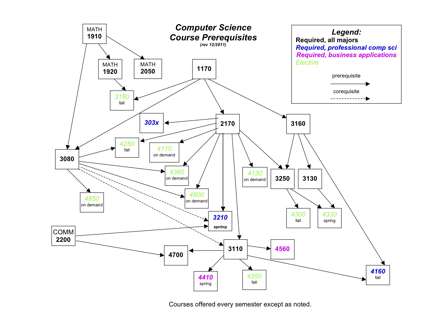
\includegraphics[]{cs_course_prereq.png}
  \caption[The course prerequisite structure for the undergraduate courses in the MTSU Computer Science Department as of December 2011.]{The course prerequisite structure for the undergraduate courses in the MTSU Computer Science Department as of May 2015.}
  \label{fig:prereq}
\end{figure}

\newpage

\begin{figure}
\begin{lstlisting}
// helloworld.cpp
#include <iostream>
using namespace std;

int main()
{
		cout << "Hello World!";

		return 0;
}
\end{lstlisting}
\caption{Example of code as figure.}\
\label{fig:code}
\end{figure}

Table \ref{tab:courses} gives an example of how captions should be centered above the table. Triple space between figures/tables and before or after any tables or figures that are inserted in the text.  For example, this text appears between figure \ref{fig:code} and table \ref{tab:courses}.  Table and figure captions should be single-spaced, and center short captions.  

\begin{table}[!b]
{\hspace{0cm}
\begin{tabular}{|p{3.5cm}|c|}
\hline \\ [-1.5ex]
\textbf{Course}    & \textbf{Credit Hours} \\
\hline \\ [-1.5ex]
CSCI 1170 & 4  \\
\hline \\ [-1.5ex]
CSCI 2170 & 4  \\
\hline \\ [-1.5ex]
CSCI 3110 & 3  \\
\hline \\ [-1.5ex]
CSCI 3130 & 4   \\
\hline \\ [-1.5ex]
CSCI 3160 & 3  \\
\hline \\ [-1.5ex]
CSCI 3210 & 3 \\
\hline \\ [-1.5ex]
CSCI 3250 & 3 \\
\hline \\ [-1.5ex]
CSCI 4160 & 3 \\
\hline \\ [-1.5ex]
CSCI 4700 & 3\\
\hline
\end{tabular}
}
\caption{Professional Computer Science Emphasis core courses as of Spring 2012}
\label{tab:courses}
\end{table}


\chapter{\textbf{REFERENCES AND CITATIONS}}
	References and citations are done using the accepted ACM reference and citation style.  This style is in accordance with both the ACM  \cite{bowman1993reasoning} and the IEEE \cite{forman2003extensive} formats for journal and paper submissions.  
	
	References are a numbered list, called the bibliography, ordered alphabetically and formatted according to the ACM reference format.  See sample references in the bibliography section of this document.  Word may try to underline links, but the correct style is NO underlining.  The Bibliography section should come immediately after the last chapter and before the appendices.  It is not a chapter, so simply center the word bibliography in bold face, all capital letters at the top of the page.
	
	A citation is given by enclosing the number of the reference in square brackets (as shown above).  Note that private communications should be acknowledged in a citation (e.g., [Pettey, private communication]), but they should not be referenced.
	
\chapter{\textbf{CHAPTERS, SECTIONS, AND SUBSECTIONS}}
Chapter numbers should be in upper case roman numerals.  The chapter number and chapter title should be on separate lines, should be in all upper case, should be bold face, and should be centered.  All section headings should be on separate lines.

\section{\underline{Primary Section Headings}}
Primary section headings should be centered on a line, bold face and underlined.  They should not be all capital letters.  Capitalize the first letter the first and last word of the heading, and capitalize the first letter of each of the other words except for articles and coordinating conjunctions and forms of to be.  

\subsection{This is a Secondary Section Heading}
Secondary section headings follow the same rules as primary section headings with the exception that they are not underlined.  

% -- Does not currently render correctly.
%\subsubsection{Tertiary Section Headings} 
%If you need a tertiary section heading, then follow the rules for primary section headings except they should be in italics and do not underline.

	
\bibliographystyle{myplain}
\clearpage
\markboth{}{}
\addcontentsline{toc}{chapter}{BIBLIOGRAPHY}
\bibliography{references}


\end{document}